\chapter{Weyl semimetals}

\section{Physical aspects}


\section{Topological description}

%TODO introductory paragraph

\subsection{3D Chern insulators}

To get a good intuition for the full topological description of Weyl semimetals, it will be useful to consider a fully insulating material with similar properties first. That is, suppose we have a three-dimensional material that is not subject to any additional symmetries. Such a material is called a 3D Chern insulator, in analogy to the 2D Chern insulator studied in Section \red{[reference]}.%TODO
This is not a semimetallic phase in the sense that there are no band crossings in the bulk; still, in some sense it can be considered a limiting case of a Weyl semimetal, where the number of Weyl points is zero.

From the Atland--Zirnbauer classification in Table \red{[reference]},%TODO
one might expect a 3D Chern insulator to be topologically trivial. However, as seen before in equation \red{[reference] (and perhaps also in 3D BHZ/Kane--Mele if I discuss this in ch. 2)},%TODO
the full topological classification of materials depends not only on the top-dimensional topology, but also on that borrowed from lower-dimensional subspaces. In the case of a 3D Chern insulator, this topology arises on two-dimensional slices of the Brillouin zone; an example of such a slice is highlighted in Figure \ref{fig:3D_Chern_insulator}.
\begin{figure}[htb!]
	\centering
	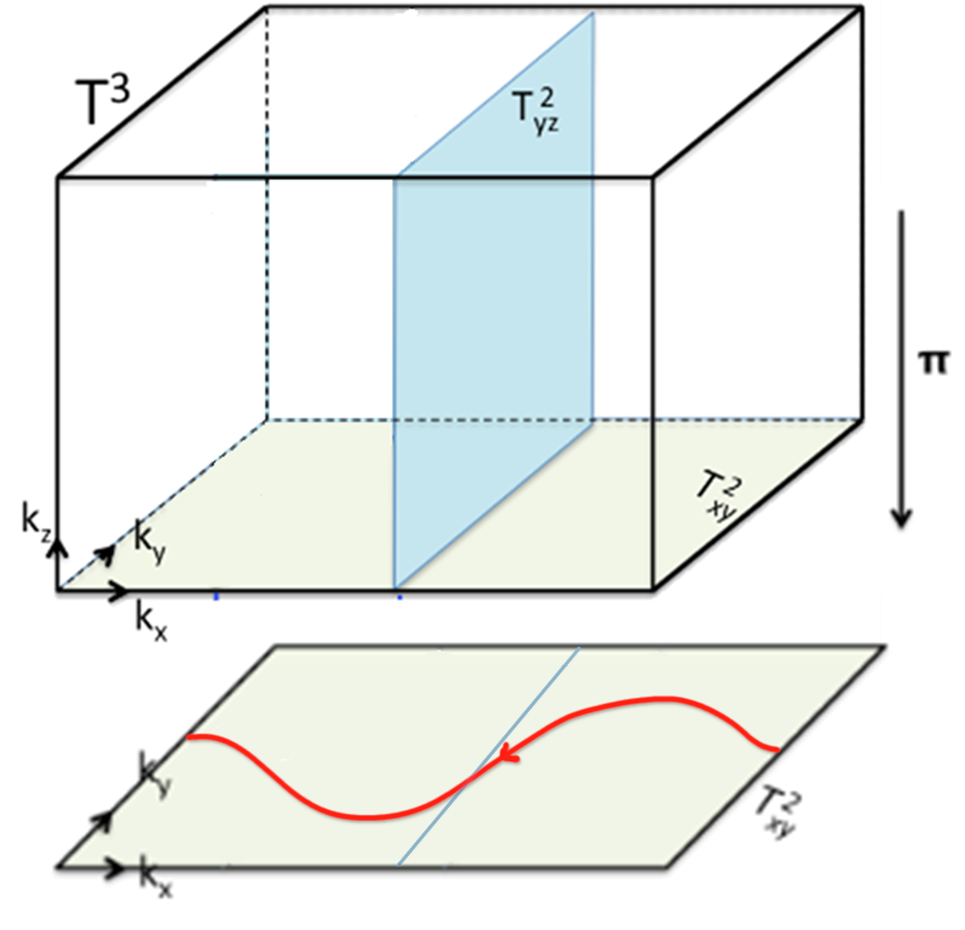
\includegraphics[width=.5\linewidth]{Images/3D_Chern_insulator}
	\caption{\red{[Temporary figure]} Three-dimensional Brillouin torus $\T^3$ of a Chern insulator, with a two-dimensional slice $\T_{yz}^2$ indicated in blue. A projection onto a surface Brillouin zone in the $xy$-direction is also shown, with an example Fermi loop of gapless states in red. In this example, the slice $\T_{yz}^2$ has a Chern number of $C_{x} = 1$, and so its projection onto the surface is a line that features one band crossing. Figure adapted from \cite{Mathai_math-review}.}
	\label{fig:3D_Chern_insulator}
\end{figure}

There are three topologically distinct ways to slice up the three-torus, all perpendicular to one of the three coordinate directions.\footnote{
	Other 2D slices exist, such as those going diagonally across, but these can all be considered linear combinations of the three ``orthogonal'' slices. To be precise, the different classes of 2D subspaces of $\T^3$ form the second homology group $H_2(\T^3)\cong\Z^3$, and this group is \emph{generated} by the orthogonal slices.}
These slices have the topology of a two-torus $\T^2$, and we can obtain a Chern number on them by integrating the Berry curvature $\Fc$ of the system over them: for example, perpendicular to the $x$ direction we obtain $C_{x} = \int_{\T_{yz}^2}\mathcal{F}$.\footnote{
	Note that it does not matter where along the Brillouin zone this $yz$-slice is taken: the Chern number is an integer, while our system is continuous. This means we can change the $x$ coordinate continuously without changing the resulting Chern number.}
This results in a classification by three distinct Chern numbers $C_x$, $C_y$ and $C_z$, and in the literature (e.g. \cites{Vanderbilt_2018}{Liu_photonic-Chern-vector}) these are commonly arranged in a so-called \emph{Chern vector}
\[
	\vb{C} = \begin{pmatrix}
		C_x \\ C_y \\ C_z
	\end{pmatrix} \in \Z^3.
\]

Importantly, these three Chern numbers are all induced by a single two-form $\Fc$. In this sense, there is an exact correspondence between topologically distinct Berry curvatures $\Fc$ and Chern vectors $\vb{C}\in\Z^3$. This is precisely what motivates the use of cohomology for classification: just like in the 2D Chern insulator, the two-form $\Fc$ can be considered an element of the second cohomology group
\begin{equation}
	H^2(\T^3)\cong\Z^3,
\end{equation}
and so this group precisely classifies the distinct topological phases of the system.\footnote{
	More fundamentally, we can associate a complex vector bundle called the \emph{valence bundle} to a gapped Hamiltonian, and the second cohomology group classifies the different complex vector bundles over a manifold.}

\subsubsection{Boundary states}

Before moving on to a system with Weyl points, it will be instructive to study the gapless modes that arise on the surface of a 3D Chern insulator with non-zero Chern vector. An example of these is illustrated in Figure \ref{fig:3D_Chern_insulator}.


\subsection{Introducing Weyl points}


\subsection{The Mayer--Vietoris sequence}


\subsection{The dual homology perspective}